\documentclass[review]{elsarticle}

\usepackage[margin=2.5cm]{geometry}
\usepackage{lineno,hyperref,booktabs,multirow,cleveref,pdflscape}
\modulolinenumbers[5]

\journal{Environmental Software and Modeling}

\bibliographystyle{APA-style}\biboptions{authoryear}

\begin{document}

\begin{frontmatter}

\title{Towards Decentralized Integration of Environmental Resources on the Web: A Resource Alignment Service}

\author[address1]{Peishi Jiang}
\author[address1]{Mostafa Elag}
\author[address2]{Luigi Marini}
\author[address2]{Liu Rui}
\author[address1]{Praveen Kumar\corref{correspondingauthor}}

\cortext[correspondingauthor]{Corresponding author}
\ead{kumar1@illinois.edu}

\address[address1]{Ven Te Chow, Hydrosystem Laboratory, Civil and Environmental Engineering, University of Illinois, Urbana, IL, USA}
\address[address2]{National Center for Supercomputing Applications, University of Illinois, Urbana, IL, USA}

\begin{abstract}
...
\end{abstract}

\begin{keyword}
Model Web \sep semantic interoperability \sep the Resource Alignment Service (RAS) 
\end{keyword}

\end{frontmatter}

\linenumbers


\section{Introduction}For decades, integrated environmental modeling has been applied in investigating the mechanism of the entire ecosystem, which becomes increasingly complex under climate change and human impact recently \citep{argent2004, laniak2013}. With the growing efforts in integrated modeling, scientists with a solo discipline background are able to access, reuse and couple reosurces (i.e.,  models and data) from various disciplines. It therefore enhances their assessment, prediction and management abilities of a complicated natural system. One of the approaches is through envisioning a world of ''Model Web'', where the functionalities of a model are exposed through web services and then integrated via the internet \citep{geller2007, geller2008, nativi2013}. As stated by \cite{nativi2013}, one of the challenges in achieving the web-serviced model integration is to ensure the 'minimal barriers to entry' or the interpoerability between the serviced resources. In this study, we aim to envision a world of 'Model Web' with emphasis on ensuring the semantic consistency of information flowing between web-serviced resources in geoscience.

The application of service-oriented architecture in environmental modeling just starts recently \citep{castronova2013, mineter2003, granell2010, goodall2011, goodall2013}. Folliwng the concept of Software as a Service (SaaS), models and data can also be exposed as web services, called as Model as a Serice (MaaS) and Data as a Service (DaaS), respectively. To achieve a world of interoperable MaaS and DaaS, the concept of ''Model Web'' was put forward by \citep{geller2008}. Later, \cite{nativi2013} explicitly defined it as ''a dynamic web of models, integrated with databases and websites, to form a consultative infrastructure where researches, managers, policy makers, and the general public can go to gain insight into ‘what if’ questions'' in initiating it under the project of the Group on Earth Observation. Several efforts have been made to draw the picture of “Model Web”. \citet{goodall2011} exposed water resource models as web services through the Open Geospatial Consortium (OGC) Web Processing Service (WPS) and demonstrated how it could be encapsulated as OpenMI(open modeling interface and environment)-compliant models. Then, they furthered the idea of servicing an OpenMI-compliant model based on WPS by considering the case of time-dependent models \citep{castronova2013}. Furthermore, an OpenMI-ESMF web service wrapper was developed to couple a climate model implemented via ESMF web service with an OpenMI-compliant hydrologic model running on a personal computer \citep{goodall2013}.

One of the key challenges in model integration communinity is the heterogeneity or long-tail property of models and data. Due to different habits of research groups or individual scientists, models developed by them would probably differ in operating system, programming language, variable name, data unit, temporal-spatial property and so forth. In the world of Model Web, a user of a web-serviced model does not need to consider the operating system or programming language of which the model is serviced and implemented because he or she only interacts with the exposed service. But the user is required to be aware of both the communication protocol the service applies and the remaining heterogeneities (e.g., variable name, data units). Otherwise, the semantic inconsistency of information flowing between services would impact the functionaility of a web serivce negatively as shown in \ref{semanticInconsistency}. To achieve a seamless integration of serviced resources, a uniform protocol and an aligning mechanism are required for information processing and ensuring reducing the semantic consistency of data flowing between serviced resources, respectively. The existing efforts described in the previous paragraph try to achieve such interoperability by applying a specific standard. For instance, apply OpenMI standard in integrating water resource models serviced by WPS \citep{goodall2011, castronova2013}. Nevertheless, the application of a certain standard or framework might not be fruitful. This is because the existence of different frameworks in different domains might imply the adoption of a specific framework in one discipline, thus complicating the online communication of serviced resources from various disciplines. For example, an OpenMI-compliant serviced model cannot talk with a serviced model embedded in Object Modeling System (OMS, \cite{david2013}) without a proper wrapper for communication between OpenMI and OMS. Furthermore, standards like OpenMI do not allow semantic mediation between variable names, prohibiting the integration of models with variables in alias names.

\begin{figure}[!htbp]
\centering
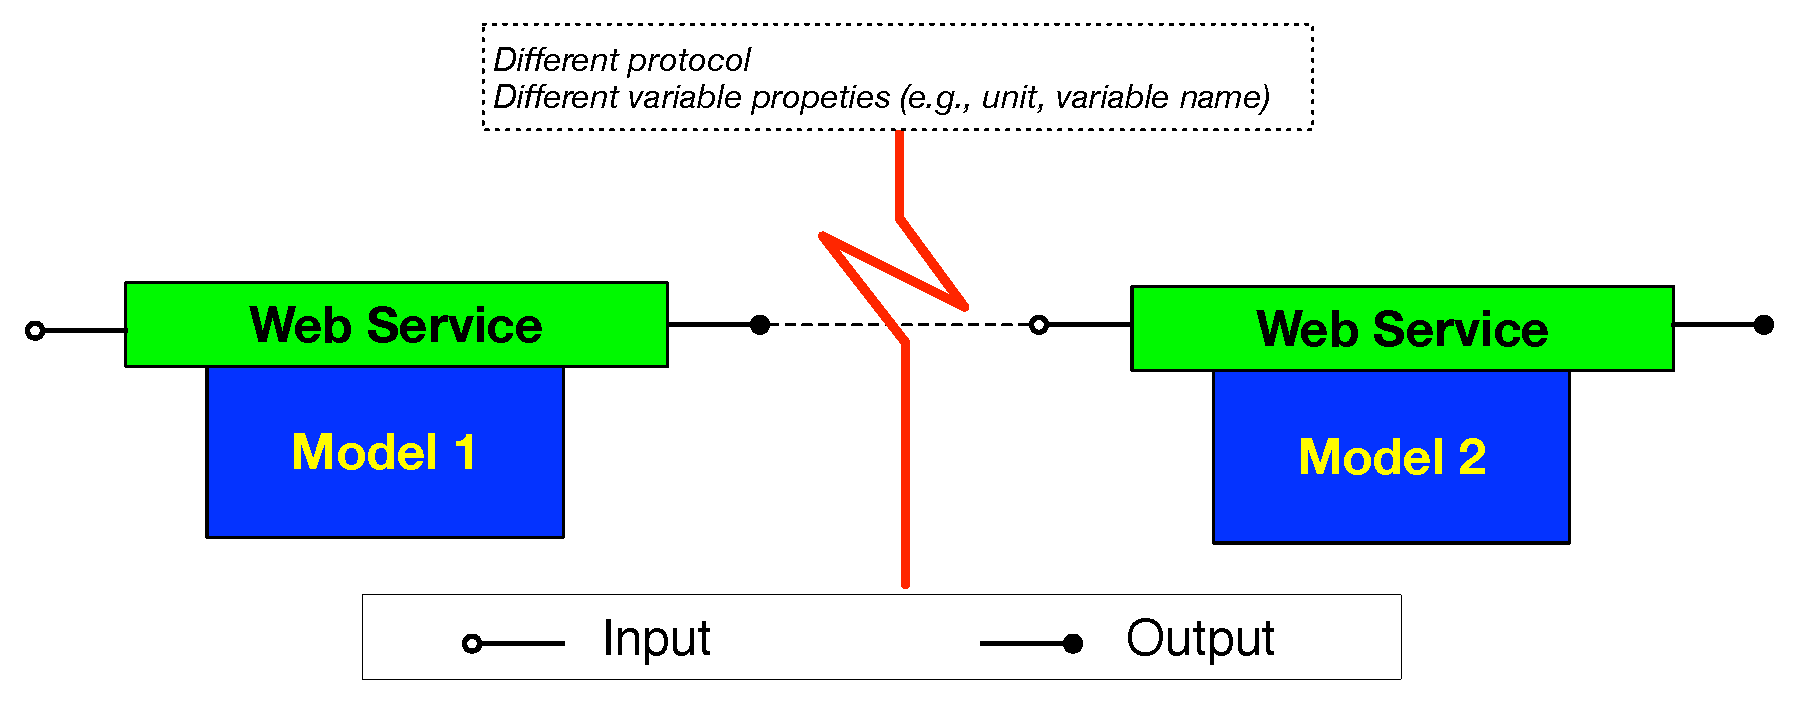
\includegraphics[scale=0.4]{../figures/figure_MaaS_misalignment.pdf}
\label{semanticInconsistency}
\caption{An illustration of the semantic inconsistency between two web serviced models.}
\end{figure}

To tackle the issue of semantic interoperability of integrating service-oriented modeling, we develop a web service named Resource Alignment Service (RAS) to ensure semantic consistency of information exchanged between MaaS over the web, including: (1) semantic mediation between variable names; (2) conversion of mismatched units; (3) temporal alignment of resource time horizon and (4) spatial alignment of resources spatial attributes. Models are implemented by the WPS, which exposes both its execution and its inputs and outputs (I/O) properties through web service. Then, RAS is utilized to align the quantities exchanging between MaaS over the webthe two types of serviced models.

In the remainder of the paper, Section 2 describes the design requirement and provides a short overview on model integration community. In Section 3, the architecture of the Resource Alignment Service (RAS is presented, including the an brief overview of GeoSemantic framework, the functionality and the components of RAS. Section 4 demonstrates the application of RAS in coupling WPS-implemented models with the input data from Clowder, an online data repository. First we create a workflow of heterogeneous collection of data and WPS-implemented models. Then, we show how RAS can seamlessly align the semantics of quantities exchanging between these resources. Finally, a brief summary is given in Section 5, with mentions on the future work. 

\section{Design Requirement and Overview}
Modeling integration in geoscience has advanced significantly these years because of the increasing collaboration between scientists or research groups from various disciplines (e.g., hydrology, geology, ecology and so on). The traditional integrated modeling approach is through tight coupling, where the initial independent models are coupled under a modeling integration application or framework. The representative integration frameworks include the Community Surface Dynamics Modeling System (CSDMS), Earth System Modeling Framework (ESMF), OpenMI standard and so forth \citep{hill2004, peckham2013, moore2005}. The CSDMS architecture employs the component-based modeling approach, where standand-alone models are encapsulated and coulped with others in a plug-and-play manner. For each model, a BMI (Basic Model Interface) file is required for recording the model's basic information and converting it into a plug-and-play component. Then, the integration process is conducted in the Component Model Interface based on all the utilities provided by CSDMS frameowork. ESMF is aimed at coupling models from Earth science (e.g., wearther and climate model), with a 'sandwich' pattern characterizing its architecture \citep{hill2004}. The user code layer contains all the model components in ESMF, which are then encapsulated in the superstructure layer aligning and connecting the input and output data between models. All the utilities for the alignment are provided in the infrastructure layer. In addition, OpenMI is an effort on model coupling in water resource community. It provides a standard interface for any new or existing models exchanging data with each other during running period. Now the OpenMI standard is adopted as a specification in the OGC.

Nevertheless, despite the advantage of the tight-coupling approach that the framework entirely controls both the data structures and processes of all parts of the model, it is difficult to couple models not following the standard or convention due to the fixed convention or standard of a framework. On the contrary, through the service-oriented loose-coupling approach, modelers only need to focus on the standardization of web interface and the protocol of data exchanging \citep{goodall2011}. As shown in \ref{tightLooseCouple}, by using web technology, the functionality of a model can be exposed as a web service with a specific protocol for data communication. In this case, by being conserved in its own hardward environment, any model requiring large data consumption or complicated configuration process can be easily coupled into any workflow or big decission system. It then also allows individual model developers or groups to maintain and update their models conveniently.

\begin{figure}[!htbp]
\centering
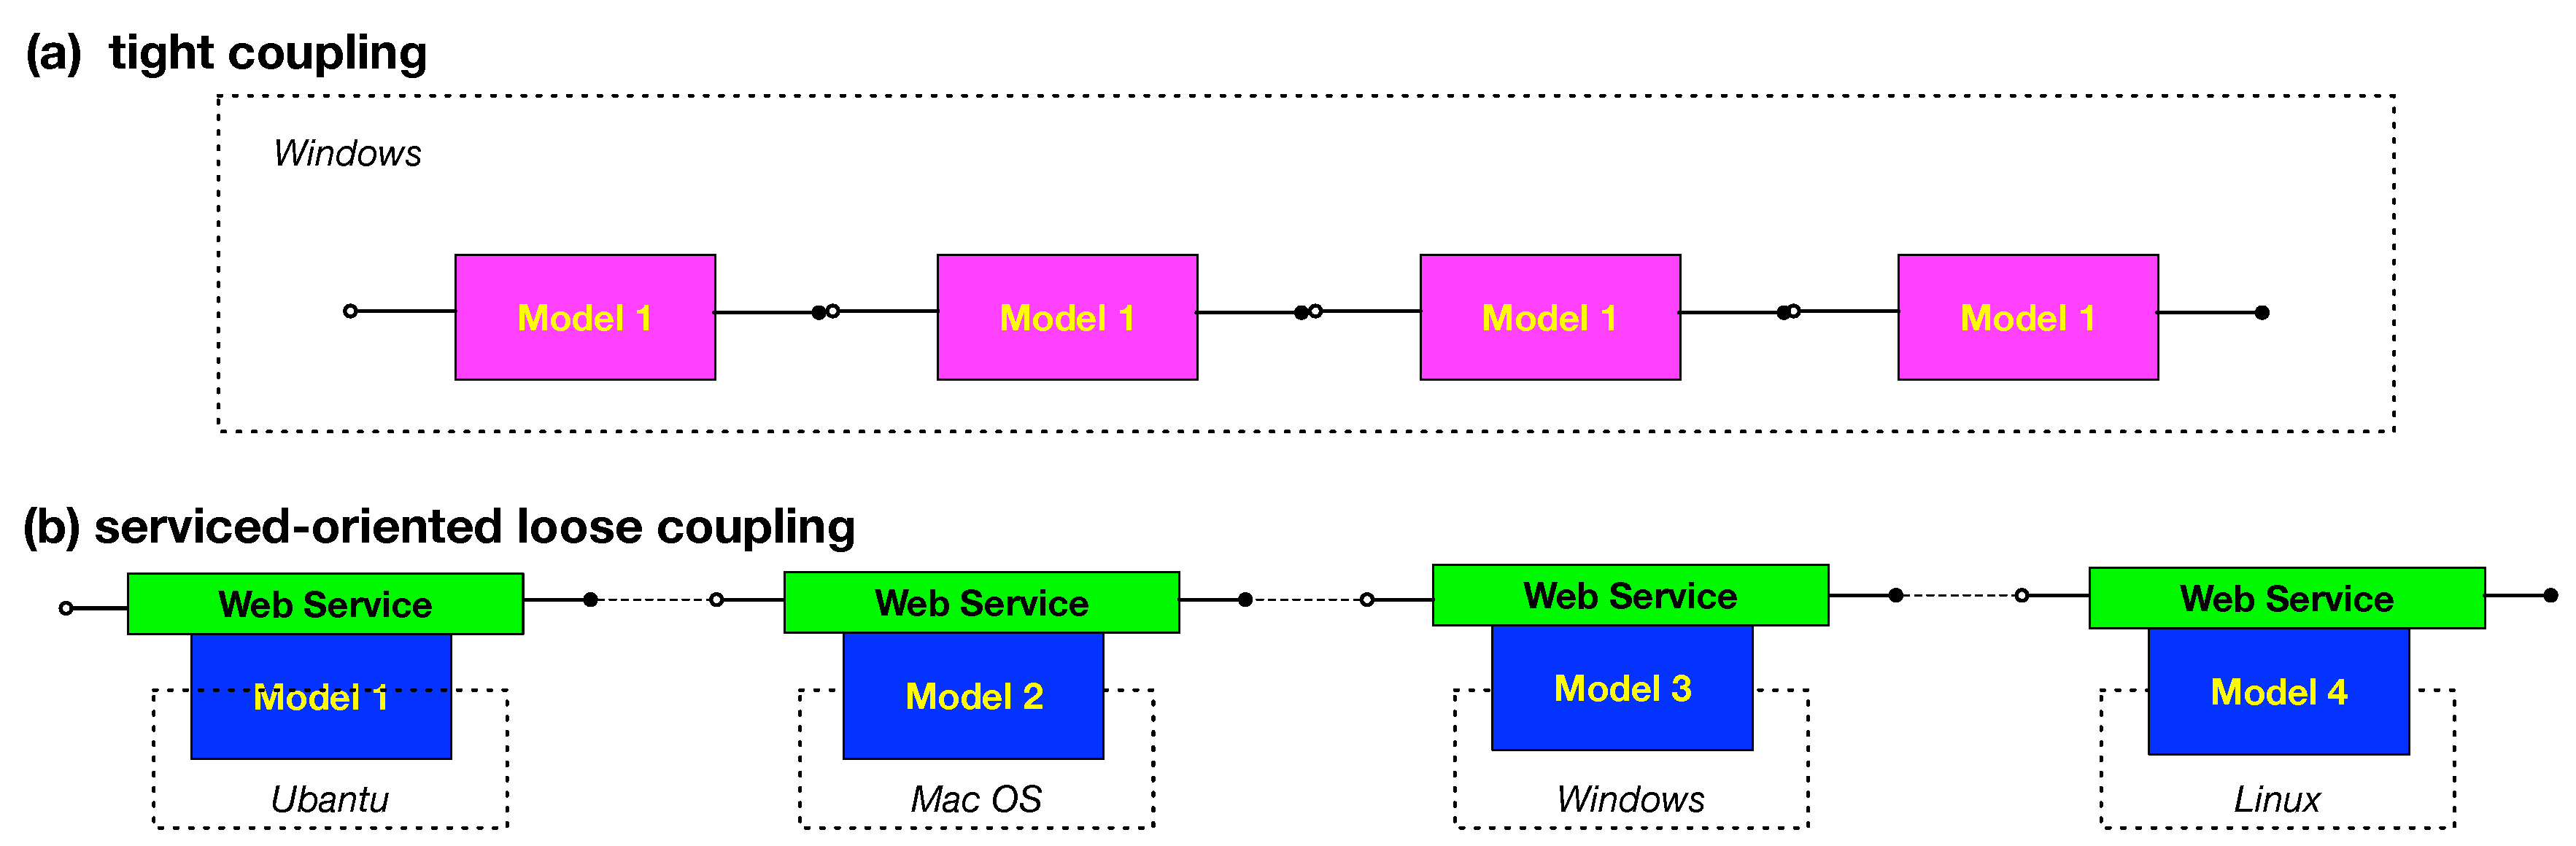
\includegraphics[scale=0.25]{../figures/figure_tight_loose_couple.pdf}
\label{tightLooseCouple}
\caption{A comparison between the tight-coupling approach and the serviced-oriented loose-coupling approach: (a) all the models are linked under the same framework and operated in the same hard environment; (b) the models implemented under various hard environment talk with each other by exposing their functionalities through web services. }
\end{figure}

Therefore, MaaS or DaaS, being able to exchange data with other serviced models over the web, requires a uniform communication protocol for information exchanging. In geoscience, the applied protocols include Water Markup Language (WaterML) and the Open Geospatial Consortium (OGC) standards for transmitting hydrologic time series data and geospatial data, respectively. WaterML is initially applied as the protocol of hydrologic data transmission in WaterOneFlow web services held by Consortium of Universities for the Advancement of Hydrologic Scienc, Inc - Hydrologic Information System (CUAHSI-HIS, \cite{valentine2007}). Now the second version of WaterML is adopted as one of the OGC standards. Furthermore, various types of standards are published by the OGC, which includes but not limited to: (1) specifications for data format such as geography markup language (GML)and keyhole markup language (KML); (2) specifications for data publication such as web coverage service (WCS), web mapping service (WMS) and web feature service (WFS); and (3) specifiations for geoprocessing such as web processing service (WPS).\cite{swain2015} provides a good review of the current open source solutions for water resources web application, most of which apply various OGC standards. In this study, as a geoprocessing standard, OGC WPS is implemented by the web serviced model, which has proven to be successfully applied in other modeling studies requiring data exchanging between services \citep{castronova2013, goodall2011, schaeffer2008,vitolo2012}.

The OGC WPS provides an approach for standardizing data processing, including three methods: GetCapabilities, DescribeProcess and Execute. The GetCapabilities method allows clients to receive a list of existing processes or models from the remote server implementing the WPS. The DescribeProcess method replies clients with the metadata of the inputs and outputs of a specific model or process. Finally, the execution of a model or process can be conducted through the Execute method based on the input values from clients. All the three methods can be requested by either HTTP POST or HTTP GET method. In this study, models are implemented by WPS, and we utilized the DescribeProcess and Execute method for retrieving the metadata specifics of the models and the model execution, respectively.



\section*{References}

\bibliography{mybibfile}

\end{document}

%%% Local Variables:
%%% mode: latex
%%% TeX-master: t
%%% End:
